\section{Proposed Methodology: RLPL}

\subsection{Improved Representation Learning}

In RLPL, the trainable and momentum networks use identical encoders for image embeddings. These embeddings are projected to a lower-dimensional space using a Multi-Layer Perceptron (MLP) in each network. The momentum network stops here, producing outputs with a dimension of 256. In contrast, the trainable network includes an additional prediction head, consisting of another MLP layer with the same dimension.

\begin{figure*}[!htbp]
    \centering
    % First subfigure
    \begin{subfigure}[b]{0.48\textwidth}
        \centering
        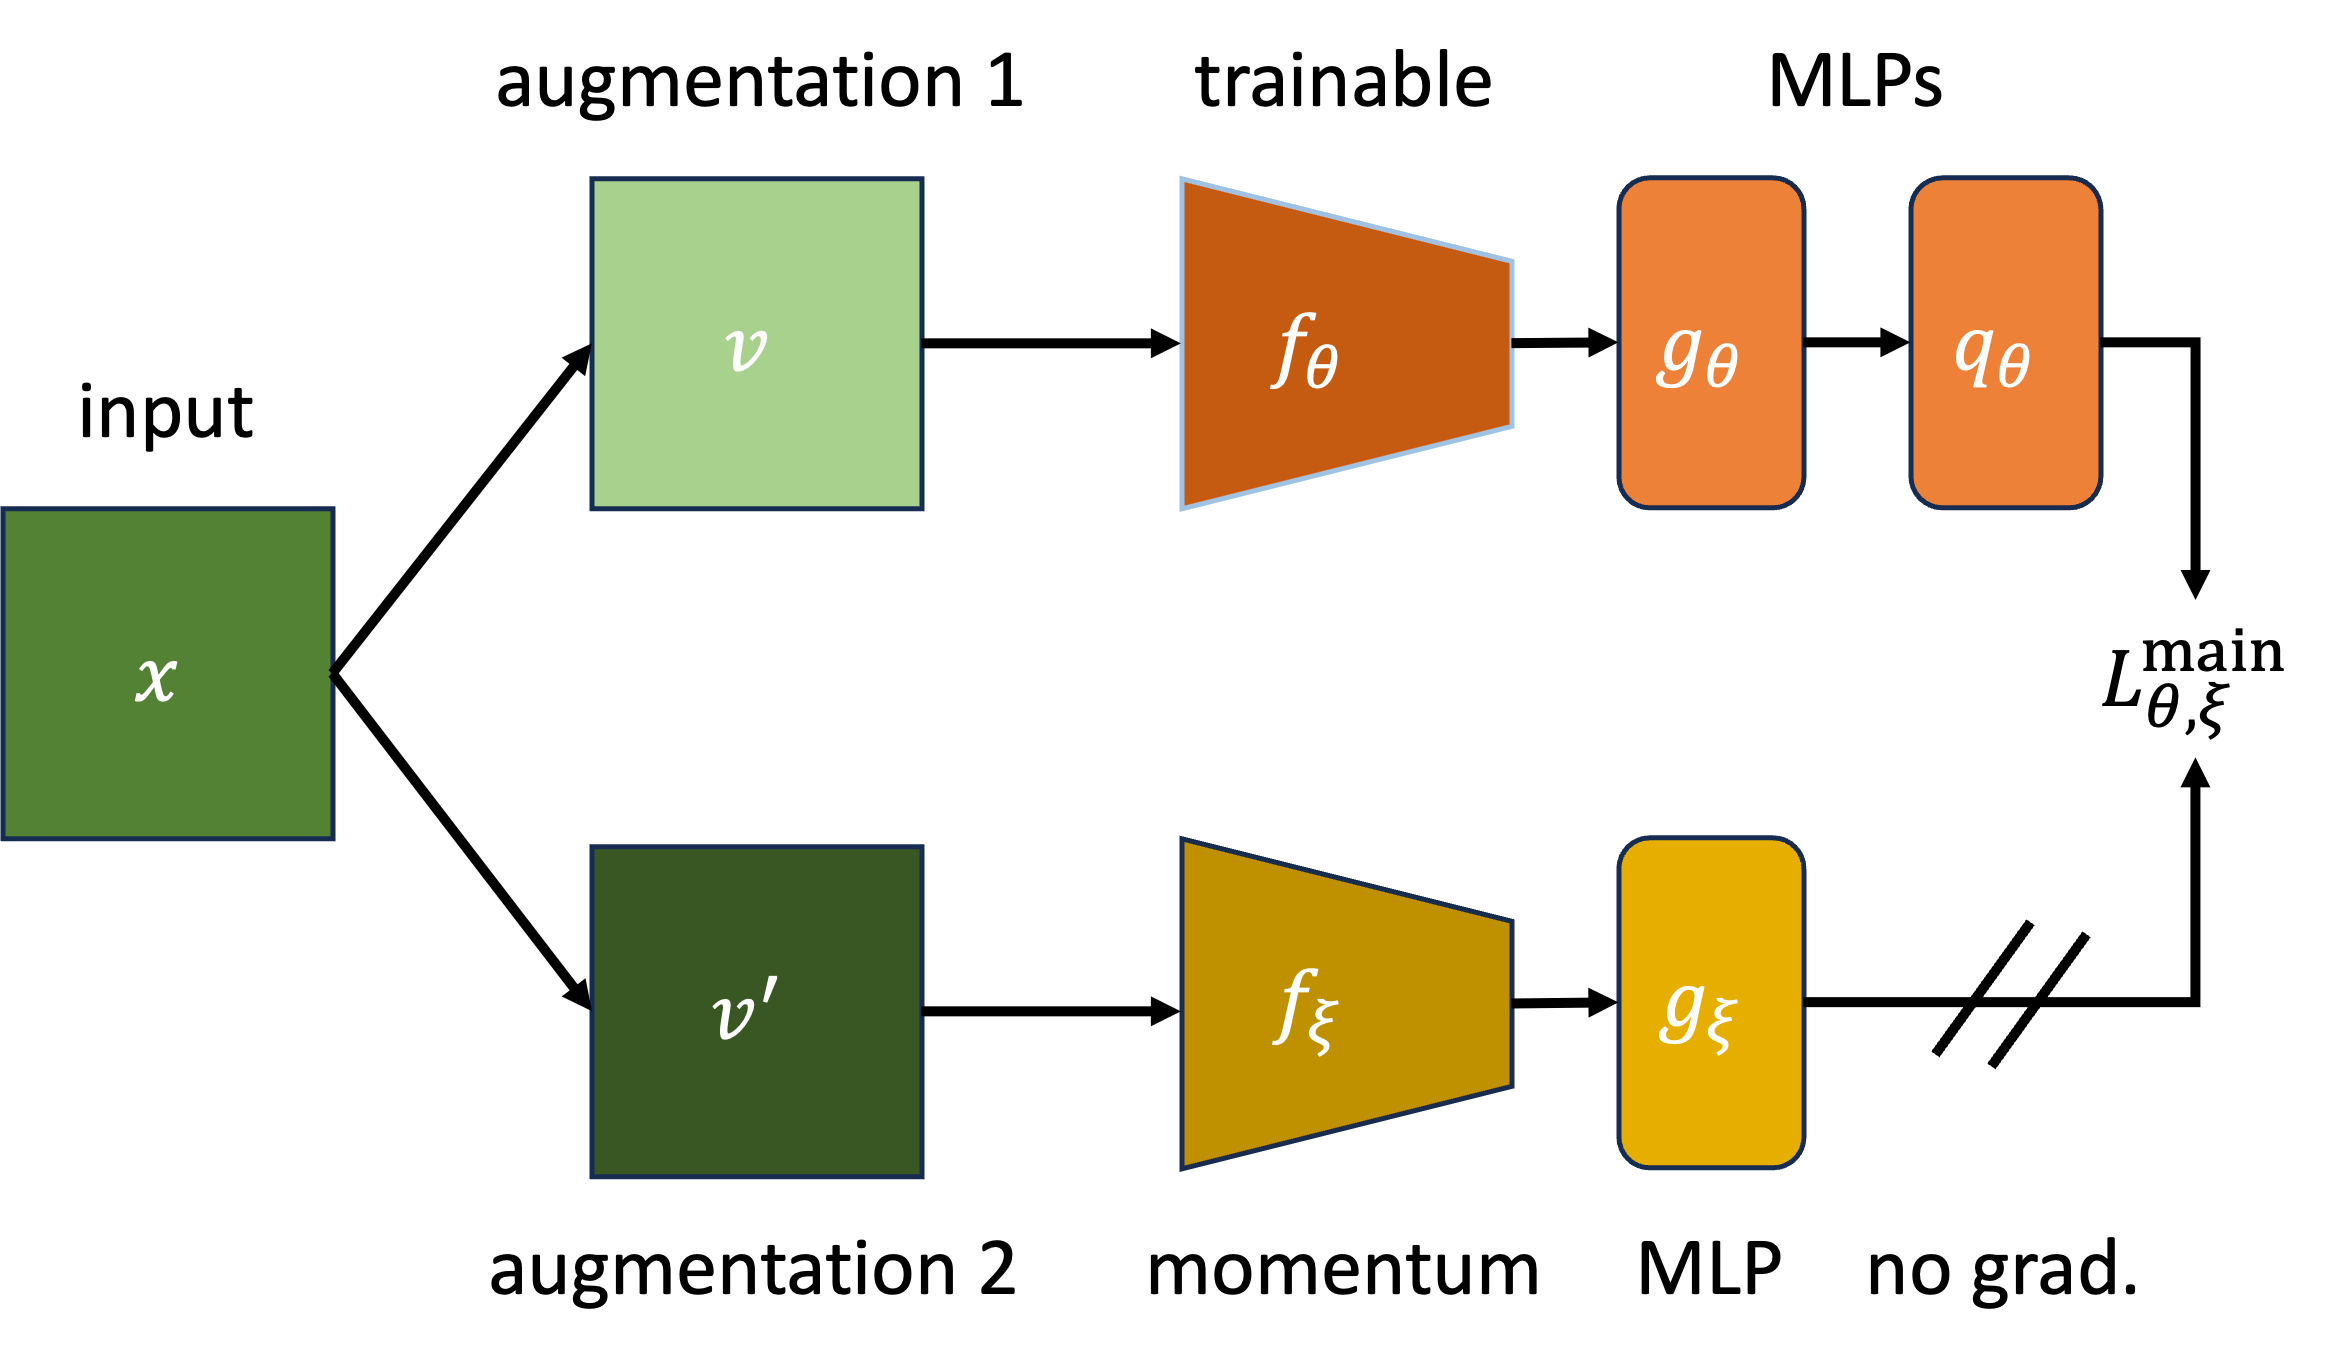
\includegraphics[width=\textwidth]{images/rl1.png}
        \caption{main loss calculation}
        \label{fig:main loss}
    \end{subfigure}
    \hspace{0.02\textwidth} % Adjust space here
    % Second subfigure
    \begin{subfigure}[b]{0.48\textwidth}
        \centering
        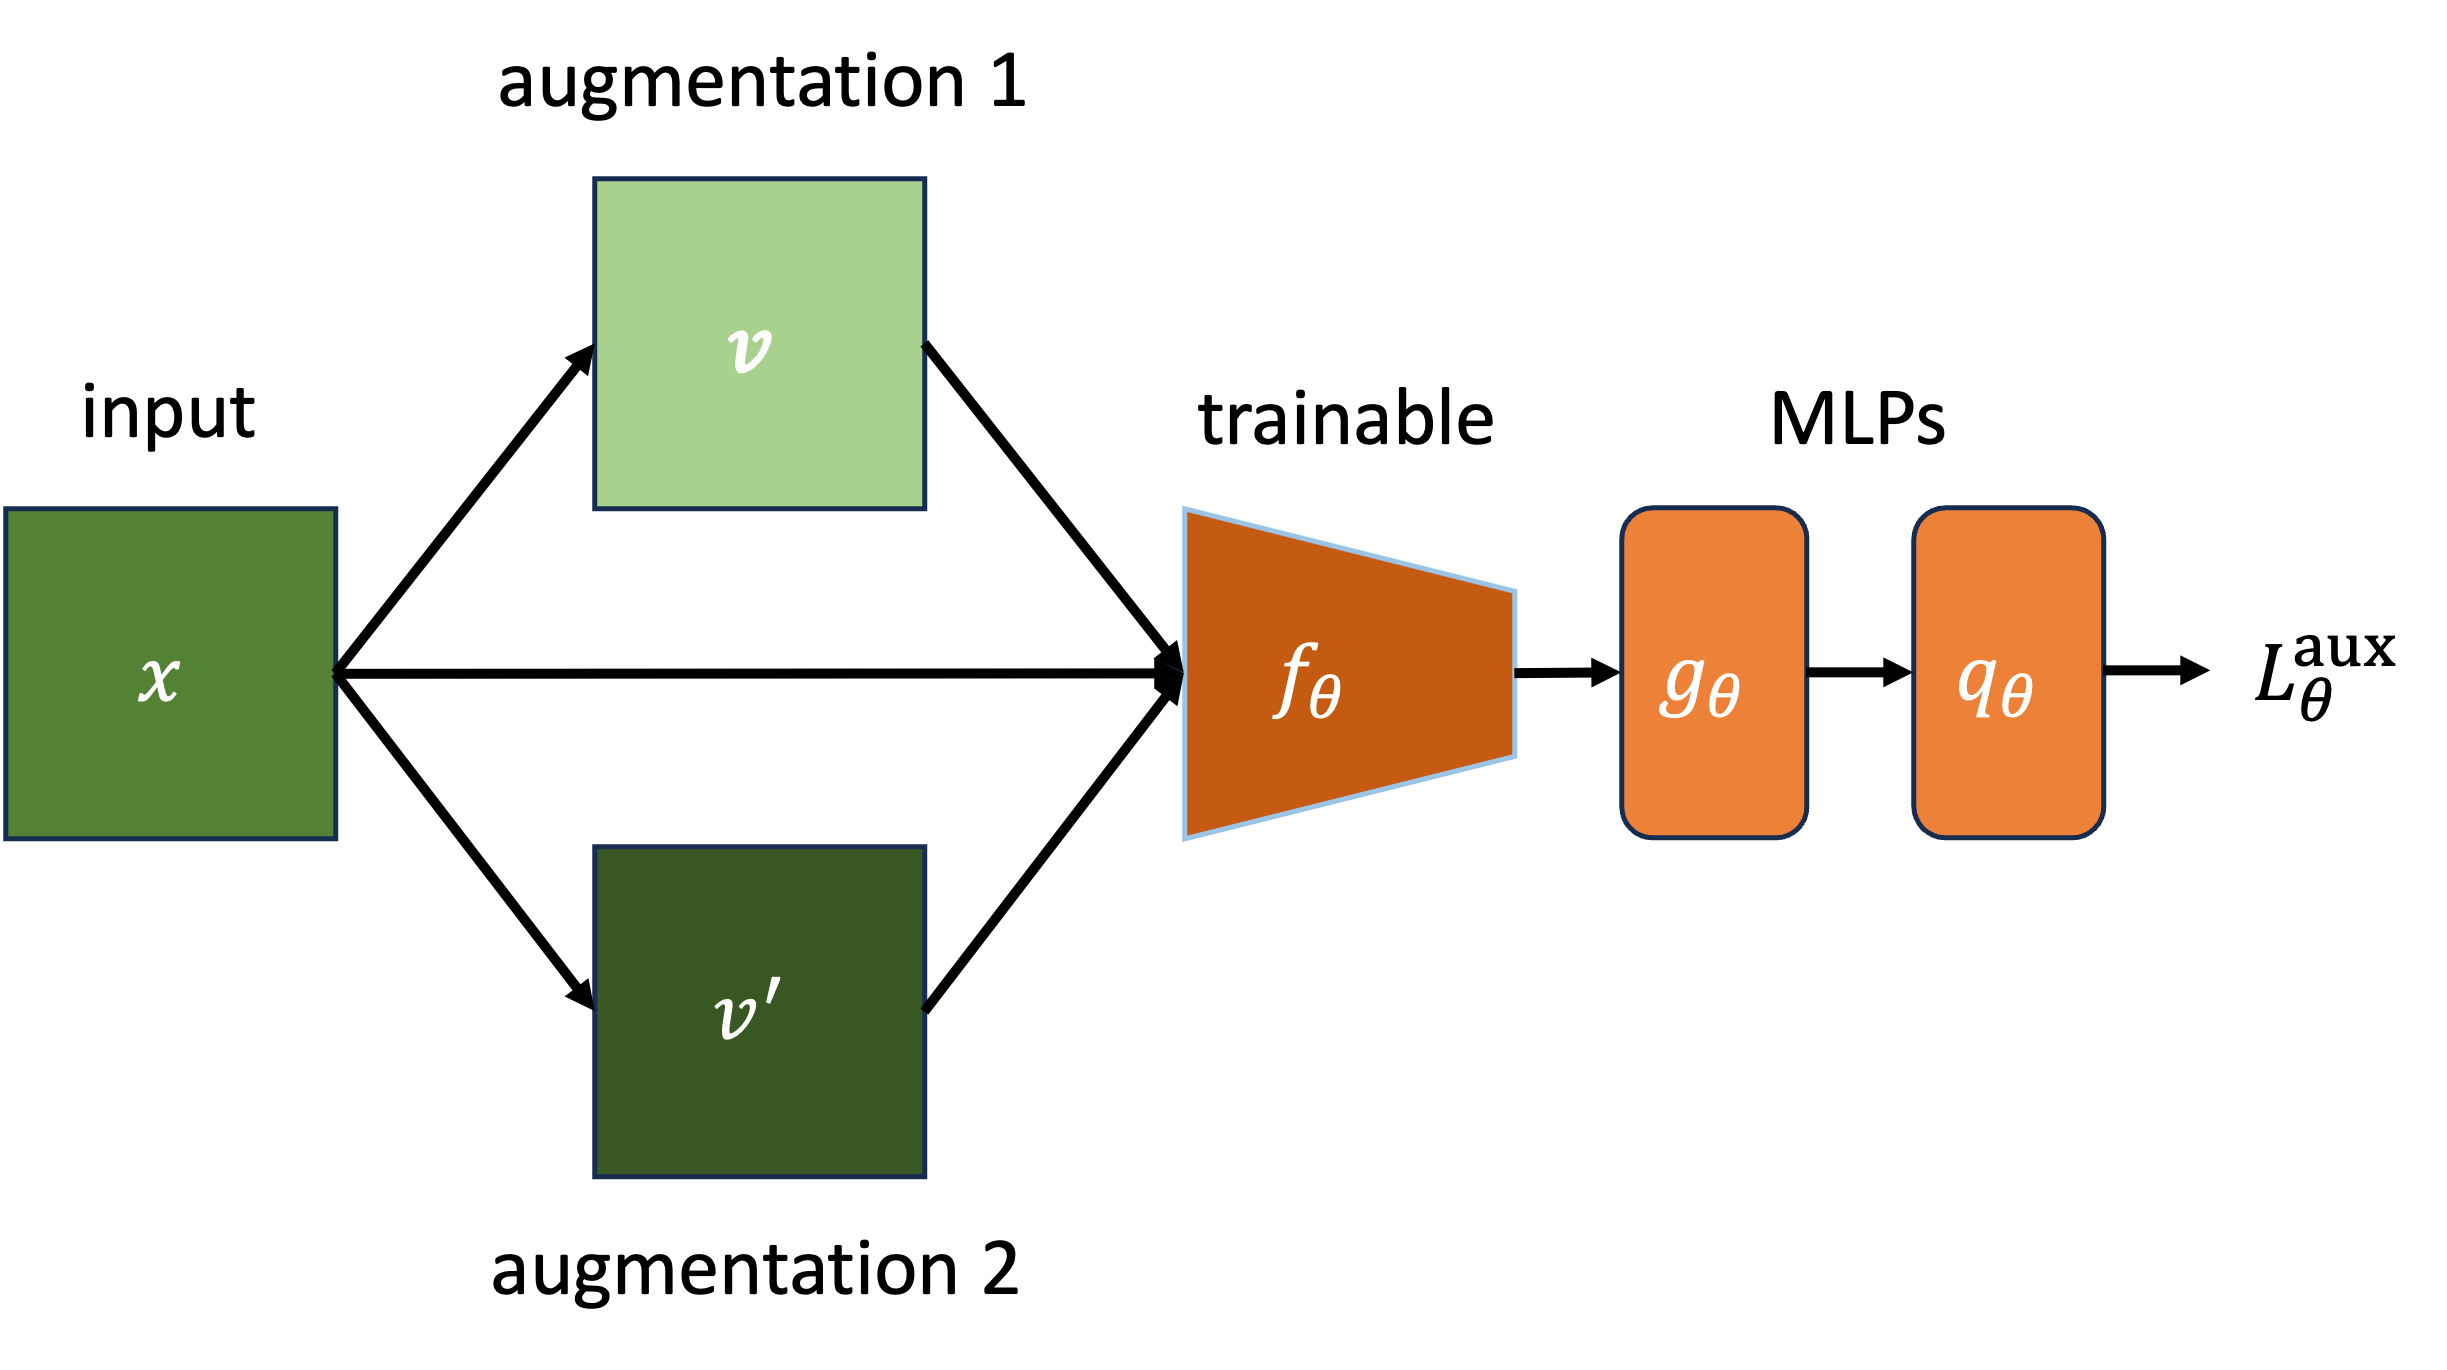
\includegraphics[width=\textwidth]{images/rl2.png}
        \caption{auxiliary loss calculation}
        \label{fig:aux loss}
    \end{subfigure}
    
    \caption{Representation learning with RLPL: \textbf{(a)} The augmented inputs are processed through both networks to compute the main loss. \textbf{(b)} The original and augmented inputs are fed into the trainable network to compute the auxiliary loss.
    }

    \label{fig:two_photos}
\end{figure*}

RLPL learns a representation $y_{\theta}$ for downstream tasks using  encoder $f_{\theta}$, a projector $g_{\theta}$, and a predictor $q_{\theta}$. The momentum network, $f_{\xi}$, with a projector $g_{\xi}$, mirrors the trainable network's architecture but updates as an exponential moving average with decay rate, $\gamma \in [0,1]$:

\begin{equation}
\xi \leftarrow \gamma \xi + (1 - \gamma) \theta.
\end{equation}

For an input image $x$, we create two augmented views $v$ and ${v}'$. The trainable network computes $y_{\theta} \triangleq f_{\theta}(v)$ and $z_{\theta} \triangleq g_{\theta}(y_{\theta})$, while the momentum network outputs $y'_{\xi} \triangleq f_{\xi}(v')$ and $z'_{\xi} \triangleq g_{\xi}(y'_{\xi})$.

We then predict $z'_{\xi}$ from $z_{\theta}$ using $q_{\theta}(z_{\theta})$, and $l_2$-normalize both $q_{\theta}(z_{\theta})$ and $z'_{\xi}$ to $\bar{q}_{\theta}(z_{\theta}) \triangleq \frac{q_{\theta}(z_{\theta})}{\| q_{\theta}(z_{\theta}) \|_{2}}$ and $\bar{z}'_{\xi} \triangleq \frac{z'_{\xi}}{\| z'_{\xi} \|_{2}}$. The loss function is the mean squared error between the normalized prediction and momentum projection (as shown in Figure \ref{fig:main loss}):

\begin{equation} \label{eq:loss}
L_{\theta, \xi} \triangleq \left\| \bar{q}_{\theta}(z_{\theta}) - \bar{z}'_{\xi} \right\|_{2}^{2} = 2 - 2 \cdot \frac{\langle q_{\theta}(z_{\theta}), z'_{\xi} \rangle}{\| q_{\theta}(z_{\theta}) \|_{2} \cdot \| z'_{\xi} \|_{2}}.
\end{equation}

To symmetrize the loss, we feed $v'$ to the trainable network and $v$ to the momentum network, computing $\tilde{L}_{\theta, \xi}$. The combined loss for optimization is:

\begin{equation}
L_{\theta, \xi}^{\text{main}} = L_{\theta, \xi} + \tilde{L}_{\theta, \xi}.
\end{equation}

To calculate the auxiliary loss, the original image goes through the online network as an additional input (as shown in Figure \ref{fig:aux loss}). For original input $x$ and augmented views $v, v'$, we obtain outputs $q_{\theta}(z_{\theta }^{x})\triangleq q_{\theta}(g_{\theta}(f_{\theta}(x)))$, $q_{\theta}(z_{\theta }^{v})\triangleq q_{\theta}(g_{\theta}(f_{\theta}(v)))$, and $q_{\theta}(z_{\theta }^{v'})\triangleq q_{\theta}(g_{\theta}(f_{\theta}(v')))$, respectively. We design an auxiliary loss that allows gradient flow during backpropagation. This auxiliary loss is combined with the main loss, weighted by a factor \(\lambda\). The momentum network stays the same, but the trainable network affects its update parameters.

We calculate the mean of two output embeddings, $\bar{q_{\theta}}(z_{\theta }^{vv'})$, from the prediction head.

\begin{equation}
\bar{q_{\theta}}(z_{\theta }^{vv'}) =  \frac{1}{2}\left ( \bar{q_{\theta}}(z_{\theta}^{v}) + \bar{q_{\theta}}(z_{\theta}^{v'}) \right )
\end{equation}
where $\bar{q_{\theta}}(z_{\theta}^{v})$ and $\bar{q_{\theta}}(z_{\theta}^{v'})$ are the batch-mean of their respective embeddings, $q_{\theta}(z_{\theta}^{v})$ and $q_{\theta}(z_{\theta}^{v'})$.

Now, we denote the auxiliary loss as $L_{\theta}^{\text{aux}}$ and it is expressed as,
\begin{equation}
L_{\theta}^{\text{aux}} = \left \| \bar{q_{\theta}}(z_{\theta}^{x}) - \bar{q_{\theta}}(z_{\theta}^{vv'})\right \|_{2}^{2}
\end{equation}

where $\bar{q_{\theta}}(z_{\theta}^{x})$ is the batch-mean of ${q_{\theta}}(z_{\theta}^{x})$.

% \begin{equation}
% \text{mean}(\bar{q_{\Theta}^{v}}(z_{\Theta}), \bar{q_{\Theta}^{v'}}(z_{\Theta})) = \frac{\bar{q_{\Theta}^{v}}(z_{\Theta}) + \bar{q_{\Theta}^{v'}}(z_{\Theta})}{2}.
% \end{equation}

Next, it is added to the main loss with a weight, $\lambda$, to obtain the total loss.

\begin{equation}
L_{\theta, \xi} = L_{\theta, \xi}^{\text{main}} + \lambda L_{\theta}^{\text{aux}}
\end{equation}

% \noindent where $\lambda$ is the weight for the auxiliary loss.

Optimization updates the trainable network parameters $\theta$ with a learning rate $\eta$, while the momentum network parameters are updated as follows:

\begin{equation}
\theta \leftarrow \text{optimizer}(\theta, \nabla_{\theta} L_{\theta, \xi}, \eta),
\end{equation}

\begin{equation}
\xi \leftarrow \gamma \xi + (1 - \gamma) \theta.
\end{equation}

After training, only the encoder $f_{\theta}$ is returned for the downstream tasks. The pseudo-code for these steps is provided in Algorithm \ref{alg:bywl}.

% \begin{figure}[t]
\begin{algorithm}[!htbp]
\caption{Representation learning with RLPL} \label{alg:bywl}
\begin{algorithmic}
\State \textcolor{pythoncomment}{\# f\_t: trainable net (backbone + projector + predictor)}
\State \textcolor{pythoncomment}{\# f\_m: momentum net (backbone + projector)}
\State \textcolor{pythoncomment}{\# lambda: weight of auxiliary loss}
\State \textcolor{pythoncomment}{\# gma: momentum update rate}

\State \text{}
\State \textcolor{pythoncomment}{\# load a minibatch x with n samples}
\State  \textcolor{pythonfunction}{for} x \textcolor{pythonfunction}{in} loader:
\State \hspace{1.1em} v1, v2 = augment(x) \textcolor{pythoncomment}{\# two random augmentations}

\State \text{}
\State \hspace{1.1em} \textcolor{pythoncomment}{\# compute embeddings}
\State \hspace{1.1em}	t, t1, t2 = f\_t(x), f\_t(v1), f\_t(v2)  , \textcolor{pythoncomment}{\# $N \times D$}

\State \text{}
\State \hspace{1.1em}	\textcolor{purpleish}{with} torch.no\_grad(): \textcolor{pythoncomment}{\# stop the gradient}
\State \hspace{2.5em}	m1, m2 = f\_m(v1), f\_m(v2) \textcolor{pythoncomment} {\# $N \times D$}

\State \text{}
\State \hspace{1.1em} \textcolor{pythoncomment}{\# calculate the losses}
\State \hspace{1.1em}	loss\_main = (loss1(t1, m2) + loss1(t2, m1)).mean()
\State \hspace{1.1em} loss\_aux = loss2(t, t1, t2)
\State \hspace{1.1em}	total\_loss = loss\_main + lambda * loss\_aux

\State \text{}
\State \hspace{1.1em} \textcolor{pythoncomment}{\# optimization step}
\State \hspace{1.1em} total\_loss.backward() 
\State \hspace{1.1em} update(f\_t.params)

\State \text{}
\State \hspace{1.1em} \textcolor{pythoncomment}{\# momentum network update}
\State \hspace{1.1em} f\_m.params = gma*f\_m.params+(1-gma)*f\_t.params

% \Ensure encoder $f_{\theta}$

\State \text{}

\State \textcolor{pythonfunction}{def} loss1(a, b):  \textcolor{pythoncomment}{\# main loss function}
\State \hspace{1.1em} a = normalize(a, dim=-1)
\State \hspace{1.1em} b = normalize(b, dim=-1)
\State \hspace{1.1em} loss = 2 - 2 * (a * b).\textcolor{pythonfunction}{sum}(dim=-1) 
\State \hspace{1.1em} \textcolor{pythonfunction}{return} loss.mean()

%\State \text{}

\State \textcolor{pythonfunction}{def} loss2(a, b, c): \textcolor{pythoncomment}{\# auxiliary loss function}
\State \hspace{1.1em}	avr\_emb = mean(b, c, dim=-1)
\State \hspace{1.1em} loss = (a - avr\_emb) ** 2)
\State \hspace{1.1em} \textcolor{pythonfunction}{return} loss.mean()
\end{algorithmic}
\end{algorithm}
% \end{figure}

\subsection{Effective Pseudo Labeling}  

For effective pseudo-labeling, let, $f_{\theta_T}$ and $f_{\theta_S}$ denote teacher and student networks initialized with parameters $\theta_T, \theta_S \leftarrow \theta$ from the pretrained encoder. Given a batch of labeled samples $(x_l, y_l) \in \mathcal{D}_l$ and unlabeled samples $x_u \in \mathcal{D}_u$, we formulate an iterative pseudo-labeling framework.

For each iteration, we first compute the student's initial loss on labeled data:

\begin{equation}
L_{s1} = \mathbb{E}_{(x_l,y_l)\sim\mathcal{D}_l}[\text{CE}(f_{\theta_S}(x_l), y_l)]
\end{equation}

For unlabeled data $x_u$, the teacher network generates soft pseudo-labels through weak augmentation $\mathcal{A}$:

\begin{equation}
\hat{y}_u = f_{\theta_T}(\mathcal{A}(x_u))
\end{equation}

To ensure quality of pseudo-labels, we filter predictions based on confidence threshold $\tau$:

\begin{equation}
\mathcal{M}_u = \{(x_u, \hat{y}_u) | \max(f_{\theta_T}(\mathcal{A}(x_u))) \geq \tau\}
\end{equation}

The teacher then learns from the filtered pseudo-labeled data:

\begin{equation}
L_u = \mathbb{E}_{(x_u,\hat{y}_u)\sim\mathcal{M}_u}[\text{CE}(f_{\theta_T}(x_u), \hat{y}_u)]
\end{equation}

After updating the student parameters using $L_u$, we measure its new performance:

\begin{equation}
L_{s2} = \mathbb{E}_{(x_l,y_l)\sim\mathcal{D}_l}[\text{CE}(f_{\theta_S}(x_l), y_l)]
\end{equation}

The effectiveness of pseudo-labeling is captured by the performance change:

\begin{equation}
\Delta L_s = L_{s2} - L_{s1}
\end{equation}

We incorporate this feedback through a meta-loss:

\begin{equation}
L_{\text{meta}} = \Delta L_s \cdot L_u
\end{equation}

The final objective for updating the teacher combines supervised learning on labeled data with the meta-loss feedback:

\begin{equation}
L_{\text{total}} = \underbrace{\mathbb{E}_{(x_l,y_l)\sim\mathcal{D}_l}[\text{CE}(f_{\theta_T}(x_l), y_l)]}_{\text{supervised loss}} + \underbrace{L_{\text{meta}}}_{\text{feedback}}
\end{equation}

This formulation creates a feedback loop where the teacher's pseudo-labeling strategy is dynamically adjusted based on the student's learning outcomes. When $\Delta L_s < 0$, indicating improved student performance, the teacher is encouraged to maintain its current strategy. Conversely, when $\Delta L_s > 0$, suggesting degraded performance, the teacher receives a stronger gradient signal to modify its approach.

The optimization proceeds iteratively:

\begin{align}
\theta_S &\leftarrow \theta_S - \eta_S \nabla_{\theta_S} L_u \\
\theta_T &\leftarrow \theta_T - \eta_T \nabla_{\theta_T} L_{\text{total}}
\end{align}

where $\eta_S$ and $\eta_T$ are learning rates for student and teacher networks respectively. After training convergence, only the teacher network is retained for deployment.

The pseudo-code for our pseudo labeling approach is provided in Algorithm~\ref{alg:PL}.

% \begin{figure}[t]
\begin{algorithm}[!htbp]
\caption{Pseudo labeling with RLPL} \label{alg:PL}
\begin{algorithmic}

\State \textcolor{pythoncomment}{\# f\_t: pretrained encoder}
\State \textcolor{pythoncomment}{\# n\_t, n\_s: teacher and student networks}
\State \textcolor{pythoncomment}{\# tau: pseudo labels threshold}

\State \text{}

\State \textcolor{pythoncomment}{\# initialize teacher and student networks}

\State n\_t = f\_t.state\_dict()
\State n\_s = f\_t.state\_dict()

\State \text{}
\State \textcolor{pythoncomment}{\# load a minibatch of labeled and unlabeled samples}
\State  \textcolor{pythonfunction}{for} x, y, x\_u \textcolor{pythonfunction}{in} loader:
\State \hspace{1.1em}	\textcolor{purpleish}{with} torch.no\_grad(): \textcolor{pythoncomment}{\# stop the gradient}
\State \hspace{2.5em} loss\_s1 = cross\_entropy(n\_s(x), y)
\State \hspace{1.1em} y\_u = n\_t(x\_u) 
\State \hspace{1.1em} \textcolor{pythoncomment}{\# filtering unlabled samples based on threshold}
\State \hspace{1.1em} x\_u, y\_u = x\_u $\left[  \text{y\_u} \geq \text{tau}\right]$, y\_u $\left[  \text{y\_u} \geq \text{tau}\right]$
\State \text{}
\State \hspace{1.1em} y\_ut = n\_t(augment(x\_u))  \textcolor{pythoncomment}{\# weak augmentation}
\State \hspace{1.1em} loss\_t = cross\_entropy(y\_ut, y\_u)
\State \hspace{1.1em} loss\_t.backward()
\State \hspace{1.1em} update(n\_s.params) \textcolor{pythoncomment}{\# student network update}

\State \text{}
\State \hspace{1.1em}	\textcolor{purpleish}{with} torch.no\_grad(): \textcolor{pythoncomment}{\# stop the gradient}
\State \hspace{2.5em} loss\_s2 = cross\_entropy(n\_s(x), y)
\State \hspace{1.1em} change = loss\_s2 - loss\_s1
\State \hspace{1.1em} meta\_loss = change * loss\_t \textcolor{pythoncomment}{\# meta-loss computation}

\State \text{} 
\State \hspace{1.1em} loss = cross\_entropy(n\_t(x), y)
\State \hspace{1.1em} total\_loss = loss + meta\_loss \textcolor{pythoncomment}{\# total loss}

\State \hspace{1.1em} total\_loss.backward()
\State \hspace{1.1em} update(n\_t.params) \textcolor{pythoncomment}{\# teacher network update}

\end{algorithmic}
\end{algorithm}
% \end{figure}
